\documentclass[a4paper]{article}
\usepackage[margin=1in]{geometry}

\usepackage{amsmath}
\usepackage{amsthm}
\usepackage{amssymb}

\usepackage[backend=biber, style=numeric]{biblatex}
\addbibresource{refs.bib}

\usepackage{graphicx, color}
\graphicspath{{fig/}}
\usepackage{algorithm, algpseudocode}
\usepackage{mathrsfs}
\usepackage{hyperref}

\usepackage{pgfplots}
\pgfplotsset{compat=1.14}
\usepgfplotslibrary{fillbetween}
\usetikzlibrary{intersections}
\usetikzlibrary{patterns}

\title{Comparación de Técnicas de Integración Numérica}
\author{Nicolás Gómez Aragón\thanks{\texttt{nicolas.gomeza@javeriana.edu.co}}}
\date{Pontificia Universidad Javeriana\\\vspace{0.5cm}\today}


\begin{document}
	\maketitle
	
	\begin{abstract}
		El propósito de este proyecto es llevar a cabo una evaluación y comparación de técnicas de integración numérica empleando funciones de prueba como referencia. Se investigarán métodos como la regla del trapecio, la regla de Simpson y la cuadratura gaussiana. Estas técnicas se implementarán en Python, y se llevará a cabo un análisis de sus resultados en términos de precisión y eficiencia computacional.
	
		\noindent\textbf{Palabras Clave:} Integración, Eficiencia, computacional.
	\end{abstract}

	\tableofcontents
	
	\section{Resumen del Proyecto}
	\label{sec:resumen}
	
	El objetivo de este proyecto es evaluar y comparar la precisión y eficiencia de varias técnicas de integración numérica utilizando funciones de prueba. Se explorarán métodos como la regla del trapecio, la regla de Simpson y la cuadratura gaussiana. Estas técnicas se implementarán en Python y se analizarán sus resultados en términos de precisión y eficiencia computacional.
	
	\section{Objetivos del Proyecto}
	\label{sec:objetivos}
	\begin{itemize}
		\item Profundizar en temas introductorios de análisis numérico y técnicas de integración numérica.
		\item Familiarizarse con implementaciones de métodos numéricos en Python para problemas de cálculo.
		\item Comprender conceptos clave como precisión y eficiencia computacional.
	\end{itemize}


	\section{Técnicas de Integración Numérica}
	\label{sec:tecnicas}
    A continuación se describen las tres técnicas de integración las cuales serán estudiadas en  este artículo.

    \subsection{Regla del Trapecio}
    La \textbf{Regla del Trapecio} es un método de aproximación numérica para calcular el valor de una integral definida. Se basa en dividir el área bajo una curva en múltiples trapecios y sumar sus áreas para estimar la integral. Para una función $f(x)$ en el intervalo $[a, b]$, la fórmula de la Regla del Trapecio se expresa de la siguiente manera:

    \[
    \int_{a}^{b} f(x) dx \approx \frac{b-a}{2} \left[f(a) + f(b)\right]
    \]
    
    donde $\frac{b-a}{2}$ es el ancho del trapecio y $\left[f(a) + f(b)\right]$ representa la suma de las alturas de los 
    extremos. Este método es simple, lo cual lo hace no muy preciso para funciones complicadas. \cite{smythnumerical} 
    
    
    \begin{center}
    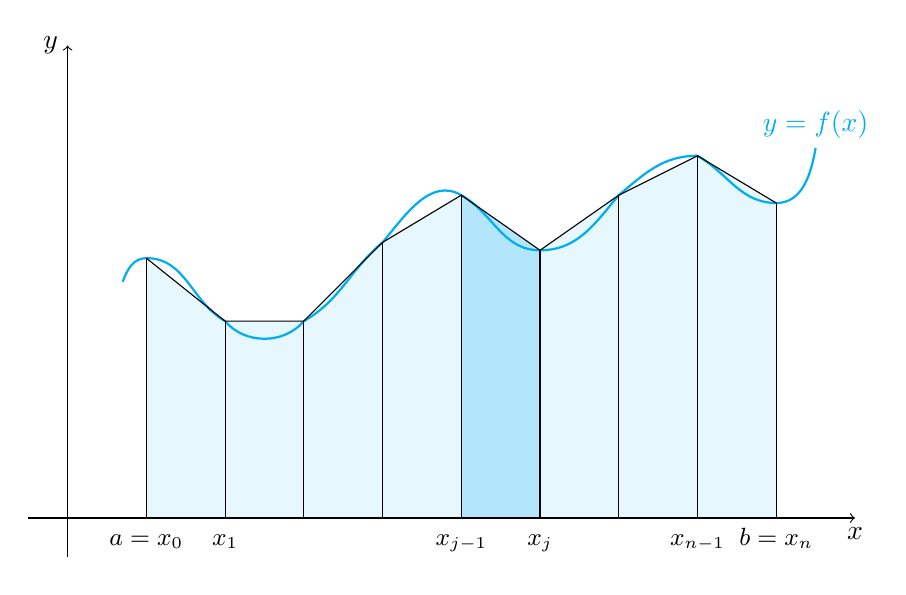
\begin{tikzpicture}
        \coordinate (p1) at (0.7,3);
        \coordinate (p2) at (1,3.3);
        \coordinate (p3) at (2,2.5);
        \coordinate (p4) at (3,2.5);
        \coordinate (p5) at (4,3.5);
        \coordinate (p6) at (5,4.1);
        \coordinate (p7) at (6,3.4);
        \coordinate (p8) at (7,4.1);
        \coordinate (p9) at (8,4.6);
        \coordinate (p10) at (9,4);
        \coordinate (p11) at (9.5,4.7);
        
        % The cyan background
        \fill[cyan!10] 
          (p2|-0,0) -- (p2) -- (p3) -- (p4) -- (p5) -- (p6) -- (p7) -- (p8) -- (p9) -- (p10) -- (p10|-0,0) -- cycle;
        % the dark cyan stripe
        \fill[cyan!30] (p6|-0,0) -- (p6) -- (p7) -- (p7|-0,0) -- cycle;
        % the curve
        \draw[thick,cyan] 
          (p1) to[out=70,in=180] (p2) to[out=0,in=150] 
          (p3) to[out=-50,in=230] (p4) to[out=30,in=220] 
          (p5) to[out=50,in=150] (p6) to[out=-30,in=180] 
          (p7) to[out=0,in=230] (p8) to[out=40,in=180] 
          (p9) to[out=-30,in=180] (p10) to[out=0,in=260] (p11);
        % the broken line connecting points on the curve
        \draw (p2) -- (p3) -- (p4) -- (p5) -- (p6) -- (p7) -- (p8) -- (p9) -- (p10);
        % vertical lines and labels
        \foreach \n/\texto in {2/{a=x_0},3/{x_1},4/{},5/{},6/{x_{j-1}},7/{x_j},8/{},9/{x_{n-1}},10/{b=x_n}}
        {
          \draw (p\n|-0,0) -- (p\n);
          \node[below,text height=1.5ex,text depth=1ex,font=\small] at (p\n|-0,0) {$\texto$};
        }
        % The axes
        \draw[->] (-0.5,0) -- (10,0) coordinate (x axis);
        \draw[->] (0,-0.5) -- (0,6) coordinate (y axis);
        % labels for the axes
        \node[below] at (x axis) {$x$};
        \node[left] at (y axis) {$y$};
        % label for the function
        \node[above,text=cyan] at (p11) {$y=f(x)$};
    \end{tikzpicture}
    \end{center}

    \subsection{Regla de Simpson}
    La \textbf{Regla de Simpson} es un método más preciso que la Regla del Trapecio para la 
    aproximación numérica de una integral definida. Utiliza polinomios de segundo grado para 
    ajustar la curva de la función. La fórmula de la Regla de Simpson se expresa de la siguiente 
    manera:
    
    \[
    \int_{a}^{b} f(x) dx \approx \frac{b-a}{6} \left[f(a) + 4f\left(\frac{a+b}{2}\right) + f(b)\right]
    \]
    
    \pagebreak
    
    Este método utiliza tres puntos (los extremos $a$ y $b$ y el punto medio que es el promedio entre ambos) para 
    ajustar una parábola, lo que lo hace más preciso que la Regla del Trapecio.\cite{srivastava2011}

    \begin{center}
        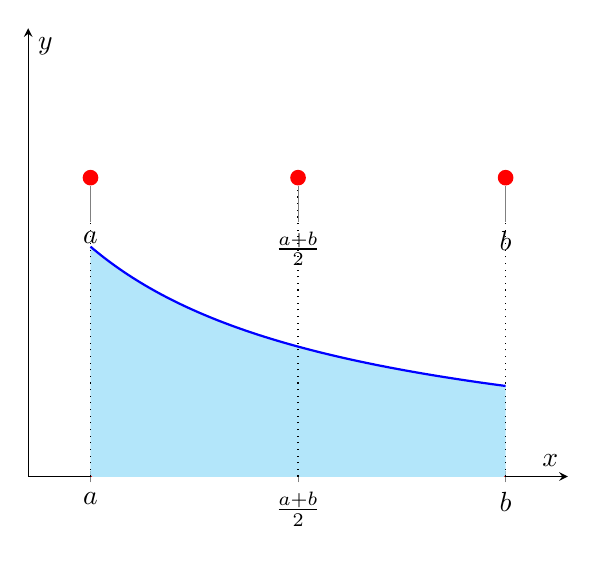
\begin{tikzpicture}
            \begin{axis}[
                axis lines=middle, 
                ytick=\empty, 
                ymax=1.5, ymin=0, xmax=2.6, xmin=0,
                xtick={0.3,1.3,2.3}, xticklabels={$a$,$\frac{a+b}{2}$,$b$},
                xlabel={$x$}, ylabel={$y$},
                every axis plot/.append style={thick}
            ]
        
            % Draw the function
            \addplot[name path=f, blue, domain=0.3:2.3, samples=100] {1/(x+1)};
        
            % Draw the Gauss-Legendre polynomial (quadratic)
            \addplot[name path=p2, red, domain=0.3:2.3] {0.5*(x-0.3)*(x-2.3)};
        
            % Fill between the function graph and the x-axis
            \addplot[cyan!30] fill between[of=f and p2];
        
            % Draw vertical lines for the interval
            \draw[dotted] (axis cs:0.3,0) -- (axis cs:0.3,1);
            \draw[dotted] (axis cs:2.3,0) -- (axis cs:2.3,1);
            \draw[dotted] (axis cs:1.3,0) -- (axis cs:1.3,1);
        
            % Place Gauss point markers
            \node[circle, fill=red, inner sep=2pt, pin=below:{$a$}] at (axis cs:0.3,1) {};
            \node[circle, fill=red, inner sep=2pt, pin=below:{$\frac{a+b}{2}$}] at (axis cs:1.3,1) {};
            \node[circle, fill=red, inner sep=2pt, pin=below:{$b$}] at (axis cs:2.3,1) {};
            
            \end{axis}
        \end{tikzpicture}
    \end{center}

    \subsection{Cuadratura Gaussiana}
    
    La \textbf{Cuadratura Gaussiana} es un método de integración numérica que utiliza nodos y pesos 
    específicos para aproximar la integral de una función en un intervalo $[a, b]$. La fórmula 
    general de la Cuadratura Gaussiana se expresa de la siguiente manera:
    
    \[
    \int_{a}^{b} f(x) \, dx \approx \sum_{i=1}^{n} w_i \cdot f(x_i)
    \]
    
    donde $w_i$ son los pesos asociados a los nodos $x_i$. La precisión de este método depende de 
    la elección de los nodos y pesos, que varían según el tipo de Cuadratura Gaussiana utilizada 
    (por ejemplo, Gauss-Legendre, Gauss-Hermite, Gauss-Laguerre, etc.).\cite{gauss_quad}
    
    \begin{center}
        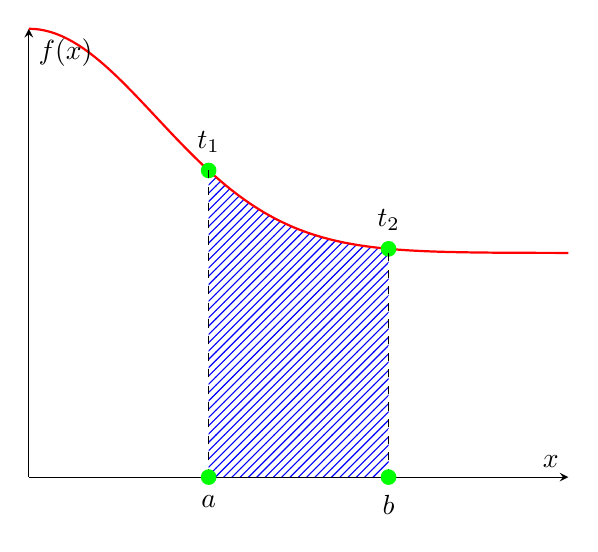
\begin{tikzpicture}
            \begin{axis}[
                axis lines=middle,
                xlabel=$x$,
                ylabel={$f(x)$},
                ticks=none,
                xmin=0, xmax=3,
                ymin=0, ymax=2,
                domain=0:3,
                samples=100,
                clip=false
            ]
        
            % Define the curve to be integrated
            \addplot[name path=f, red, thick] {exp(-x^2) + 1};
        
            % Define the integration area
            \path[name path=axis] (axis cs:0,0) -- (axis cs:3,0);
        
            % Draw the shaded area
            \addplot[pattern=north east lines, pattern color=blue] fill between[of=f and axis, soft clip={domain=1:2}];
        
            % Draw the Gauss points
            \node[shape=circle, fill=green, inner sep=2pt, label=above:{$t_1$}] at (axis cs:1, {exp(-1^2) + 1}) {};
            \node[shape=circle, fill=green, inner sep=2pt, label=above:{$t_2$}] at (axis cs:2, {exp(-2^2) + 1}) {};
        
            % Draw the vertical dashed lines
            \draw[dashed] (axis cs:1,0) -- (axis cs:1, {exp(-1^2) + 1});
            \draw[dashed] (axis cs:2,0) -- (axis cs:2, {exp(-2^2) + 1});
        
            % Draw the interval [a,b]
            \node[shape=circle, fill=green, inner sep=2pt, label=below:{$a$}] at (axis cs:1, 0) {};
            \node[shape=circle, fill=green, inner sep=2pt, label=below:{$b$}] at (axis cs:2, 0) {};
        
            \end{axis}
        \end{tikzpicture}
    \end{center}

    En la figura anterior se representa la aproximación de cuadratura gaussiana para la integración numérica de la función $f(x) = e^{-x^2} + 1$ en el intervalo $[1, 2]$. Los puntos verdes, $t_1$ y $t_2$, corresponden a los nodos de Gauss, donde se evalúa la función. Las líneas discontinuas verticales marcan las posiciones de estos nodos. La región sombreada ilustra el área bajo la curva de $f(x)$ que se aproxima mediante polinomios que pasan por los puntos de Gauss, lo cual permite una estimación precisa de la integral de la función en el intervalo dado.



    \section{Funciones de Prueba}
	\label{sec:funciones}
    Para evaluar y probar los métodos de integración numérica, consideramos las siguientes tres 	
    funciones de prueba:

    \begin{enumerate}
    
      \item \textbf{Función Polinómica:}
       Esta función polinómica simple se puede integrar analíticamente, lo que la hace útil para 
       comparaciones de precisión.
      \begin{equation}
      f(x) = x^2 + 3x - 5
      \end{equation}
    
      \item \textbf{Función racional:}
       Se optó por esta función por su simplicidad y la presencia de un término logarítmico en la 	
       integral, lo cual proporciona un buen ejemplo para evaluar la precisión de nuestras técnicas 
       numéricas. Además, la integración de funciones racionales es una práctica común en análisis 
       numérico y nos permite explorar cóo nuestros métodos se desempeñan en este contexto.
      \begin{equation}
      f(x) = \frac{1}{x + 1}
      \end{equation}

       \item \textbf{Función Trigonométrica:}
       La naturaleza trigonométrica de esta función nos permite probar cómo manejan los métodos
       numéricos el comportamiento oscilatorio.
      \begin{equation}
      f(x) = \sin(x)
      \end{equation}
    
    \end{enumerate}

    \subsection{Soluciones analíticas}
    Solucionamos analíticamente las funciones para encontrar las soluciones exactas a sus integrales para poder establecer un punto de comparacion con las soluciones de los métodos de integración.

    \begin{enumerate}
      \item \textbf{Función polinómica:}
      \begin{equation}
      \int x^2 \, dx = \frac{1}{3}x^3 + C
      \end{equation}
      Donde \(C\) es una constante de integración.

      \item \textbf{Función racional:}
      \begin{equation}
      \int \frac{1}{x + 1} \,dx = \ln|x + 1| + C 
      \end{equation}
    
      \item \textbf{Función trigonométrica:}
      \begin{equation}
      \int \sin(x) \, dx = -\cos(x) + C
      \end{equation}
    \end{enumerate}

    \subsection{Reemplazo en intervalo}

    Tomando como punto de referencia un intervalo determinado para las tres funciones podemos
    comparar más fácilmente las soluciones analíticas con las funciones por métodos computacionales para 
    su posterior análisis.

    Así con esto, el intervalo será \( [0, 2] \) para las integrales definidas.

    \begin{enumerate}
        \item \textbf{Función polinómica:}
        \begin{equation}
        \int_{0}^{2} x^2 \, dx = \frac{1}{3}x^3 \Big|_{0}^{2} = \frac{1}{3}(2^3 - 0^3) = \frac{8}{3} = 2.666666667
        \end{equation}
    
        \item \textbf{Función racional:}
        \begin{equation}
        \int_{0}^{2} \frac{1}{x + 1} \,dx = \ln|x + 1| \Big|_{0}^{2} = \ln(3) - \ln(1) = \ln(3) = 1.098612289
        \end{equation}
    
        \item \textbf{Función trigonométrica:}
        \begin{equation}
        \int_{0}^{\pi} \sin(x) \, dx = -\cos(x) \Big|_{0}^{\pi} = -\cos(\pi) + \cos(0) = 2
        \end{equation}
    \end{enumerate}
    
    \section{Implementación en Python}
	\label{sec:python}
    La implementaciones de cada técnica de integración numérica en el lenguaje de 
    programación Python pueden encontrarse en el \href{https://github.com/nicolasgomeza7/tecnicasIntegracion}{repositorio}.
    
    \section{Resultados}    
    
    \subsection{Eficiencia}

    En este contexto eficiencia se refiere a la capacidad de un método o algoritmo de integración computacional para realizar cálculos de manera rápida y efectiva, minimizando el tiempo necesario para obtener resultados. La eficiencia es un aspecto crucial en la elección y aplicación de métodos de integración, ya que puede tener un impacto significativo en el rendimiento y la utilidad de las soluciones obtenidas.
    
    En términos de eficiencia, medida como el tiempo de cálculo, se observaron los siguientes resultados:
    
   \subsubsection{Función Trigonométrica}
    \begin{itemize}
        \item Método más rápido: Trapezoidal (6.3e-05 segundos).
        \item Orden de eficiencia: Trapezoidal $>$ Simpson $>$ Gaussiano.
    \end{itemize}
    
    \subsubsection{Función Polinomial}
    \begin{itemize}
        \item Método más rápido: Trapezoidal (2.1e-05 segundos).
        \item Orden de eficiencia: Trapezoidal $>$ Simpson $>$ Gaussiano.
    \end{itemize}
    
    \subsubsection{Función Racional}
    \begin{itemize}
        \item Método más rápido: Trapezoidal (1.5e-05 segundos).
        \item Orden de eficiencia: Trapezoidal $>$ Simpson $>$ Gaussiano.
    \end{itemize} 

    
    \subsection{Precisión}
    Precisión en este contexto se refiere a la capacidad de un método computacional para obtener 
    resultados que se acerquen de manera significativa a la solución analítica o teórica. La precisión es 
    esencial en la evaluación de la confiabilidad de los resultados obtenidos mediante técnicas de
    integración, ya que nos permite determinar cuán cercanos están a las respuestas exactas.

    En cuanto a la precisión, medida como la cercanía a la solución analítica, se obtuvieron los 
    siguientes hallazgos:

    \subsubsection{Función Polinomial}
    \begin{itemize}
        \item Método más rápido: Trapezoidal con un tiempo de 1.2e-05 segundos.
        \item Seguido de: Simpson con una diferencia de 1.1130218505859372e-06 segundos respecto al método más rápido
        \item Seguido de: Gaussiana con una diferencia de 0.003229856491088867 segundos respecto al método más rápido
        \item Aproximación más cercana: Gaussiana.
    \end{itemize} 

    \subsubsection{Función Racional}
    \begin{itemize}
        \item Método más rápido: Trapezoidal con un tiempo de 1e-05 segundos.
        \item Seguido de: Simpson con una diferencia de 1.2056732177734367e-06 segundos respecto al método más rápido.
        \item Seguido de: Gaussiana con una diferencia de 0.00025463104248046875 segundos respecto al método más rápido.
        \item Aproximación más cercana: Gaussiana. 
    \end{itemize}

    \subsubsection{Función Trigonométrica}
    \begin{itemize}
        \item Método más rápido: Trapezoidal con un tiempo de 4e-05 segundos.
        \item Seguido de: Simpson con una diferencia de 5.061111450195309e-06 segundos respecto al método más rápido.
        \item Seguido de: Gaussiana con una diferencia de 1.9073486328125e-06 segundos respecto al método más rápido.
        \item Aproximación más cercana: Gaussiana. 
    \end{itemize}
    
    \subsection{Análisis de resultados}
    Se observa una clara compensación entre eficiencia y precisión en los métodos evaluados. Mientras que los métodos Trapezoidal y Simpson son más rápidos, el método Gaussiano proporciona resultados más precisos. 
    
    La elección del método adecuado dependerá del equilibrio entre la necesidad de eficiencia (tiempo de cálculo) y precisión. Para funciones complejas o donde se requiere alta precisión, el tiempo adicional requerido por el método Gaussiano puede ser justificado, mientras que para respuestas rápidas con menor necesidad de precisión, los métodos Trapezoidal o Simpson pueden ser más adecuados.
    
    \section{Aplicaciones}
    En esta parte del proyecto se mostrarán 3 proyectos de aplicación donde los métodos computacionales, en especial los de integración juegan un rol determinante.

    \subsection{Problema de manejo de embalses}
    En el proyecto este proyecto de Universidad Autónoma de México (UNAM), se aborda una aplicación práctica de las técnicas de integración numérica en el ámbito de la ingeniería hidrológica. El estudio se enfoca en el uso de esquemas de integración numérica de Newton - la Regla del Trapecio, Simpson 1/3 y Simpson 3/8 - para calcular el volumen de almacenamiento en el embalse de la presa "Las Cruces", que forma parte de un proyecto hidroeléctrico. Este análisis resalta la relevancia de los métodos numéricos en la resolución de problemas complejos en el campo de la hidrología de superficie, una disciplina crucial en el diseño y manejo de infraestructuras hidráulicas.

    Uno de los aspectos centrales del proyecto es la aplicación de la ecuación diferencial de continuidad para modelar el tránsito de avenidas en embalses, un enfoque que refleja la importancia de los métodos numéricos en el análisis hidrológico moderno. Además, se realiza una comparativa entre los volúmenes estimados mediante estos métodos de integración y los obtenidos a través de un programa de la Comisión que emplea una integración a través de rectángulos. Este contraste demuestra no solo la precisión de los métodos de Newton, sino también su utilidad práctica en escenarios de ingeniería real, proporcionando una base sólida para la toma de decisiones en proyectos de gran envergadura.\cite{newton_method}

    \subsection{OpenGeoSys}
    El proyecto OpenGeoSys (OGS) se presenta como una iniciativa científica de código abierto para la simulación numérica de procesos termo-hidro-mecánico-químicos (THMC) en medios porosos. Empleando principalmente el Método de Elementos Finitos (FEM), OGS proporciona un marco numérico flexible para abordar problemas multifacéticos con aplicaciones en geociencia e hidrología. 

    El modelado de procesos en OGS ha sido relevante en diversas áreas de la ingeniería y aplicaciones geocientíficas desde los 70s, abordando problemas como la consolidación del suelo, construcción de presas y exploración de campos de petróleo y gas. Los avances en estudios experimentales y teóricos sobre los efectos de temperatura, hidráulica, mecánica y química en medios porosos fracturados se han acelerado en las últimas dos décadas, impulsados por la necesidad de evaluar el rendimiento y la seguridad de los depósitos de residuos nucleares de alto nivel.

    Para la evaluación del rendimiento y la seguridad a largo plazo de un repositorio de residuos nucleares en una formación geológica profunda, es crucial garantizar el aislamiento de un repositorio subterráneo. Se necesita predecir numéricamente los procesos de transporte de solutos bajo condiciones acopladas que involucran estabilidad mecánica, carga térmica de los residuos de alto nivel y química en las aguas subterráneas. Con el rápido desarrollo de la tecnología informática, es posible analizar problemas geocientíficos complicados de manera acoplada utilizando códigos numéricos modernos. Sin embargo, entender estos procesos acoplados basados en datos experimentales disponibles e implementar los algoritmos desarrollados en los códigos numéricos sigue siendo un gran desafío para los científicos, requiriendo cooperación interdisciplinaria e interactiva.\cite{geosys}

    El sitio oficial del proyecto es \href{https://www.opengeosys.org/#:~:text=OpenGeoSys%20,the%20fields%20of%20regionals}{página web} y el código de este puede encontrarse en el siguiente \href{https://gitlab.opengeosys.org/ogs/ogs}{repositorio}.
    
    \subsection{Algoritmos en el Desarrollo de Motores de Juegos}
    Otra faceta de los métodos numéricos se encuentra el desarrollo de motores para videojuegos, incluyendo el Método de Euler, el Método de Verlet y el Método de Runge-Kutta para la integración numérica. La detección de colisiones y cómo se equilibra la simplicidad y precisión en este proceso, incluyendo el uso de volúmenes de límites geométricos y el algoritmo GJK son temas ampliamente estudiados, así como el cálculo de los puntos de contacto utilizando el Algoritmo de Sutherland-Hodgman para determinar la respuesta a colisiones.\cite{serranoalgos}
    
    Un ejemplo de la importancia de los métodos de integración numérica y aprendizaje profundo en el desarrollo de videojuegos es el estudio realizado en el juego \textit{DOOM}. En el artículo "Playing Doom with SLAM-Augmented Deep Reinforcement Learning", se explora un enfoque innovador para el aprendizaje de políticas en juegos 3D, utilizando un modelo de agente que incorpora conceptos semánticos y abstracciones. Este modelo se apoya en la Red de Aprendizaje Profundo Q (DQN) y mejora el procesamiento de entornos 3D complejos al añadir detalles sobre objetos y elementos estructurales, así como la localización del jugador. 

    El estudio demuestra cómo la introducción de mapas en el modelo DQN estándar, que proporcionan información agregada sobre el entorno 3D alrededor del personaje, mejora la eficacia del aprendizaje en \textit{DOOM}. Estos mapas permiten al agente mantener información sobre áreas observadas anteriormente y construir un modelo agregado del entorno 3D, lo cual es crucial en el escenario de duelo a muerte de \textit{DOOM}, donde el objetivo es eliminar tantos oponentes como sea posible. La investigación subraya los beneficios de las representaciones en el aprendizaje de políticas, ofreciendo perspectivas para mejorar el rendimiento y la escala de los algoritmos de aprendizaje en entornos 3D más allá de "DOOM".\cite{doommethods}
     
    \section{Conclusiones}
    \label{sec:Conclusiones}
    Este proyecto ha explorado la utilidad y aplicación de algunos métodos de integración numérica, subrayando su importancia en una amplia gama de campos científicos. La integración numérica es fundamental en áreas donde las soluciones analíticas son difíciles o imposibles de obtener, como en la física computacional, la ingeniería, la economía, la modelización de fenómenos naturales y procesos industriales, entre otros.

    A través del análisis de la Regla del Trapecio, la Regla de Simpson y la Cuadratura Gaussiana, hemos demostrado cómo cada técnica tiene sus propias ventajas y limitaciones, dependiendo del contexto. El método del Trapecio y la Regla de Simpson, debido a su mayor eficiencia en términos de tiempo de cálculo, son especialmente útiles en situaciones donde se requiere una respuesta rápida y la precisión absoluta no es crítica, mientras que la Cuadratura Gaussiana, con su mayor precisión, es invaluable en investigaciones científicas y aplicaciones técnicas donde la exactitud es primordial.
    
    Este proyecto no solo ha proporcionado una comparación detallada de la eficiencia y precisión de estos métodos, sino que también ha brindado una plataforma para familiarizarse con su implementación en Python, así como también algunas de sus aplicaciones a nivel científico e industrial.
    
    En conclusión, los métodos de integración numérica son herramientas poderosas y flexibles en el análisis numérico. Su comprensión y correcta aplicación son cruciales para resolver problemas complejos en el mundo moderno, y este proyecto ha planteado una introducción a su entendimiento, proporcionando familiaridad y un entorno para su aplicación en diferentes escenarios.    

    \printbibliography

\end{document}

